\documentclass[10pt,twocolumn]{article}

\usepackage[a4paper,margin=0.7in]{geometry}
\usepackage[T1]{fontenc}
\usepackage[utf8]{inputenc}
\usepackage{lmodern}
\usepackage{graphicx}
\usepackage{booktabs}
\usepackage{array}
\usepackage{longtable}
\usepackage{hyperref}
\usepackage{enumitem}
\usepackage{xcolor}
\usepackage{caption}

\hypersetup{
  colorlinks=true,
  linkcolor=blue,
  citecolor=blue,
  urlcolor=blue
}

\title{\textbf{GazePose-Context: Multimodal Context Inference for Adaptive XR Training in Unity and Meta Quest}}
\author{
  Lavanya D. \and Varun Siddaraju \and Dr. Alexandra Kitson
}
\date{}

\begin{document}
\maketitle

\begin{abstract}
Adaptive extended reality (XR) systems need to respond to user attention, disengagement, and task flow without requiring explicit user input. This paper presents GazePose-Context, a Unity-based XR prototype that infers user context during a simple training task by combining gaze, head pose, body posture, hand interaction, and spatial context signals. The system organizes processing into three layers: sensor abstraction, context inference, and XR adaptation. Multimodal signals are synchronized into a shared SignalFrame, transformed into modality-specific feature vectors, fused through interpretable rules, and stabilized with a hysteresis-based state machine to estimate four context states: Engaged, Distracted, Transitioning, and Idle. These states drive lightweight adaptive behaviors such as subtle focus reinforcement, redirection prompts, next-step support, and rest-oriented controls. The current implementation targets Meta Quest deployment using Unity 2022.3.62f1, OpenXR 1.14.3, Meta XR All-in-One SDK 201.0.0, and OVRPlugin 1.201.0. This paper reports the current implementation status in the repository, integrates the reference figures from the earlier draft, and prepares the manuscript in paper-ready LaTeX format while leaving explicit placeholders only where verified literature and user-study results are still missing.
\end{abstract}

\textbf{Keywords:} XR, adaptive interfaces, multimodal interaction, gaze, body pose, hand tracking, context inference, Meta Quest

\section{Introduction}
Immersive systems are increasingly expected to understand what a user is doing and to react in ways that support attention, task completion, and comfort. In XR training environments, these expectations are especially strong because users often move between focus, transition, confusion, interruption, and rest without explicitly announcing those states. A system that can infer context from ongoing behavior can potentially guide the user without interrupting task flow or overloading the interface.

Most current XR experiences still rely on explicit UI actions, hard-coded task triggers, or isolated interaction signals. A single modality rarely captures the full structure of user behavior. Gaze alone cannot distinguish between task engagement and exploratory scanning. Hand interaction alone cannot represent attention drift. Body posture or locomotion alone can be ambiguous without knowing where the user is looking or whether they are interacting with task objects. This motivates a multimodal approach to context inference.

This paper presents \textbf{GazePose-Context}, an XR prototype developed in Unity for Meta Quest-class devices. The prototype combines gaze-related cues, head pose, posture and joint movement, hand pinch interactions, and spatial boundary context to infer one of four user states: \textit{Engaged}, \textit{Distracted}, \textit{Transitioning}, and \textit{Idle}. These states are then mapped to lightweight adaptive behaviors inside a simple training simulation. The task environment is intentionally constrained: the user sorts three virtual objects into matching receptacles. This simple task reduces gameplay complexity while making attention, object interaction, and task transitions easier to observe and interpret.

The current paper reflects the actual repository status rather than the earlier unfinished draft. The implementation side is now substantially stronger: the repository contains the signal schema, synchronization, feature extraction, rule-based fusion, state hysteresis, XR adaptation, and logging pipeline. The empirical evaluation side remains partially pending because the final participant study results and the full verified bibliography were not recoverable from the local draft assets.

The contributions of this work are:
\begin{enumerate}[leftmargin=1.2em]
  \item A three-layer XR architecture for multimodal context inference and adaptive support.
  \item A synchronized runtime signal representation combining gaze, head, body, hand, and spatial context data.
  \item An interpretable rule-based context engine that estimates Engaged, Distracted, Transitioning, and Idle states with confidence scores.
  \item A boundary-aware adaptation layer that changes feedback strategy based on user state and spatial setup.
  \item A logging and evaluation design aligned with a within-subjects adaptive-vs-baseline user study.
\end{enumerate}

\section{Related Work}
The current paper is positioned at the intersection of XR sensing, multimodal interaction, context-aware adaptation, and immersive training support. The reference list provided for this paper shows four especially relevant lines of work: eye tracking and attention measurement in XR, multimodal interaction pipelines, body and hand tracking for embodied interaction, and context-aware adaptation in immersive systems.

\subsection{Gaze and Attention Modeling}
Eye tracking has become one of the most important sensing channels in XR because it provides a direct proxy for user attention, fixation stability, and target selection. Moreno-Arjonilla et al. survey the broader state of eye tracking in virtual reality and help position gaze sensing as a mature but still evolving foundation for adaptive immersive systems \cite{moreno2024}. Work comparing gaze accuracy and precision between real-world and VR conditions is also relevant because the present system depends on AOI-level reliability rather than only coarse orientation cues \cite{gazecomparison2020}. At the feature-extraction level, the current implementation uses an Identification by Velocity Threshold (I-VT) style fixation detector with a 30 degrees/second velocity threshold and an 80 ms minimum fixation duration, following a standard fixation-identification approach in eye-tracking literature \cite{salvucci2000}. The use of dwell ratio and saccade rate as secondary features follows the same general logic of aggregating gaze dynamics into interpretable behavioral features.

Attention modeling in XR is also increasingly multimodal. Long et al. combine EEG and eye tracking for detecting internal and external attention in virtual reality, showing the broader research trend toward richer attention inference beyond gaze alone \cite{long2024}. In a more intervention-oriented direction, Selaskowski et al. demonstrate that gaze-based attention refocusing in VR can be used as part of adaptive training and therapeutic support, which is directly relevant to the adaptive redirection logic in the present work \cite{selaskowski2023}.

\subsection{Workload and User Evaluation}
Multimodal interaction in XR has expanded well beyond controller-only paradigms. Rakkolainen et al. provide a scoping review of technologies for multimodal interaction in extended reality, which supports the design decision to combine gaze, hand, body, and head channels in a single system rather than treating them separately \cite{rakkolainen2021}. Kim et al. similarly frame XR interaction as an evolution from controllers toward broader multimodal input ecosystems, reinforcing the relevance of layered sensing and fusion architectures \cite{kim2026}. On the adaptation side, Davari and Bowman explicitly address context-aware adaptation in extended reality, making their work one of the closest conceptual neighbors to the present system \cite{davari2024}. Ramiotis and Mania's CONTEXT-GAD work is especially relevant because it links gaze-aware adaptation with context-sensitive dwell modeling in immersive interaction \cite{ramiotis2025}.

The embodied components of the present pipeline are also supported by recent work on posture and hand tracking. Bustamante et al. show the value of skeleton-based posture recognition for applied settings \cite{bustamante2025}, while Neidhardt et al. demonstrate the use of VR-based body tracking for musculoskeletal training applications \cite{neidhardt2023}. For the hand-interaction channel, Lei et al. present a sensor-fusion approach for precise hand tracking in VR \cite{lei2023}. Together, these works support the inclusion of posture, joint movement, and hand interaction features in the current system.

The evaluation plan uses NASA-TLX as a secondary measure of subjective workload, which is standard for human factors and interactive systems evaluation \cite{hart1988}. In the planned study, NASA-TLX is intended to complement behavioral metrics such as context detection accuracy, task completion time, and sorting errors.

\subsection{Pending Reference Integration}
The current reference set now supports the core framing of the paper: gaze sensing in VR \cite{moreno2024,gazecomparison2020}, multimodal attention and interaction \cite{long2024,rakkolainen2021,kim2026}, embodied posture and hand tracking \cite{bustamante2025,neidhardt2023,lei2023}, and context-aware adaptation in XR \cite{davari2024,ramiotis2025}. As the paper is further refined, these references should be verified and formatted against the target venue's bibliography style.

\section{Problem Statement and Research Questions}
The core problem addressed in this paper is how to infer task-relevant user context in real time during immersive interaction and use that inference to adapt XR behavior without requiring manual status input from the user.

The primary research question is:

\textbf{RQ1.} Can multimodal XR signals be fused in real time to infer task-relevant user context during a simple immersive training activity?

The secondary research question is:

\textbf{RQ2.} Does context-aware adaptive support improve task performance and subjective experience relative to a non-adaptive baseline?

These questions are operationalized through a sorting task in which the user places three objects into corresponding receptacles. The task provides a controlled environment in which gaze targets, hand interactions, posture changes, and task transitions can be observed with relatively low confound from gameplay complexity.

\begin{figure*}[t]
  \centering
  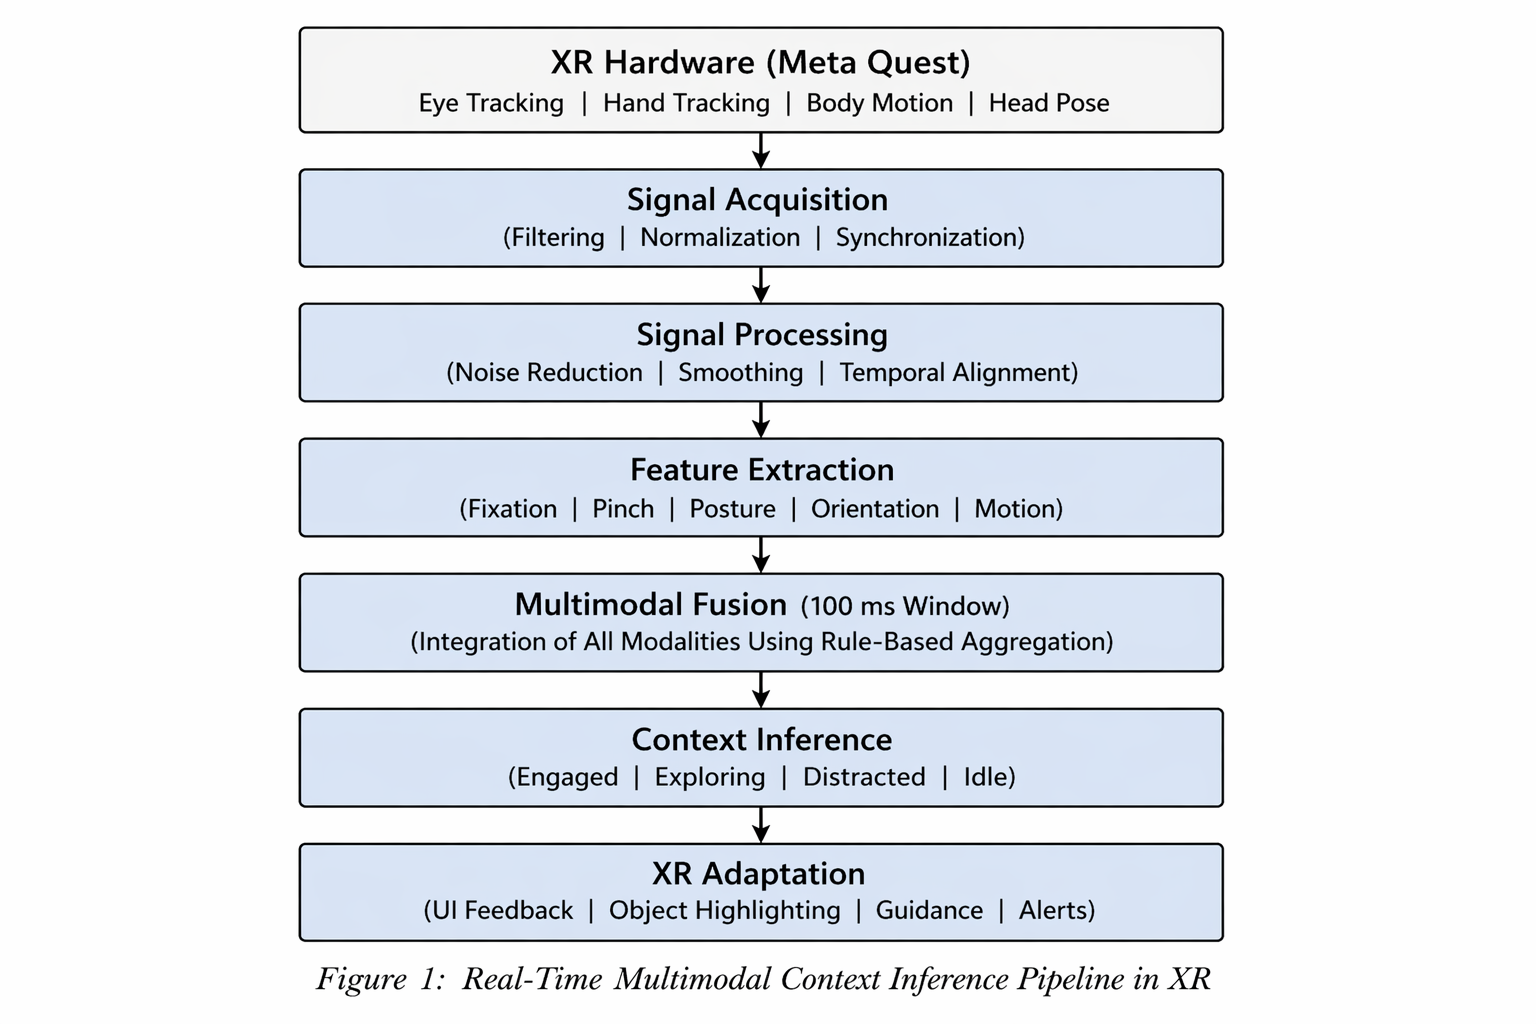
\includegraphics[width=0.9\textwidth]{figures/figure1_pipeline.png}
  \caption{Reference pipeline figure from the earlier draft. The current repository still matches the overall multimodal processing flow, but the final paper text now maps it into the repository's three-layer structure: Sensor Abstraction, Context Engine, and XR App Shell.}
  \label{fig:pipeline}
\end{figure*}

\section{System Architecture}
The implemented prototype follows a three-layer architecture:
\begin{enumerate}[leftmargin=1.2em]
  \item \textbf{Sensor Abstraction Layer}
  \item \textbf{Context Engine}
  \item \textbf{XR App Shell}
\end{enumerate}

This architecture mirrors the planning documents and is also reflected in the current repository structure.

\subsection{Layer 1: Sensor Abstraction}
The sensor abstraction layer collects raw runtime signals and writes them into a synchronized data structure. The core contract between Layer 1 and Layer 2 is the \texttt{SignalFrame} struct. Each frame contains timestamped gaze, head, body, hand, spatial, and derived context fields, including timestamp, gaze origin and direction, fixation metadata, AOI hit, head position and forward vector, head-gaze divergence, posture class, spine angle, joint velocity, pinch states, interaction counts, nearest object distance, posture mode, boundary type, locomotion delta, context state, confidence, previous state, state hold duration, transition count, and nearest interactable reference.

The synchronizer emits a shared frame every 100 ms using \texttt{InvokeRepeating}, yielding a 10 Hz context-processing cadence in the current repository implementation.

\subsection{Layer 2: Context Engine}
The context engine transforms each synchronized frame into higher-level multimodal features, estimates a candidate context state through rule-based fusion, and stabilizes the result through a temporal state machine. This layer contains the main research logic of the prototype.

\subsection{Layer 3: XR App Shell}
The XR application layer consumes the current state and boundary context and selects the appropriate adaptive behavior. This layer is intentionally separated from the context engine so that inference logic remains independent of Unity-specific UI and scene objects.

\begin{figure*}[t]
  \centering
  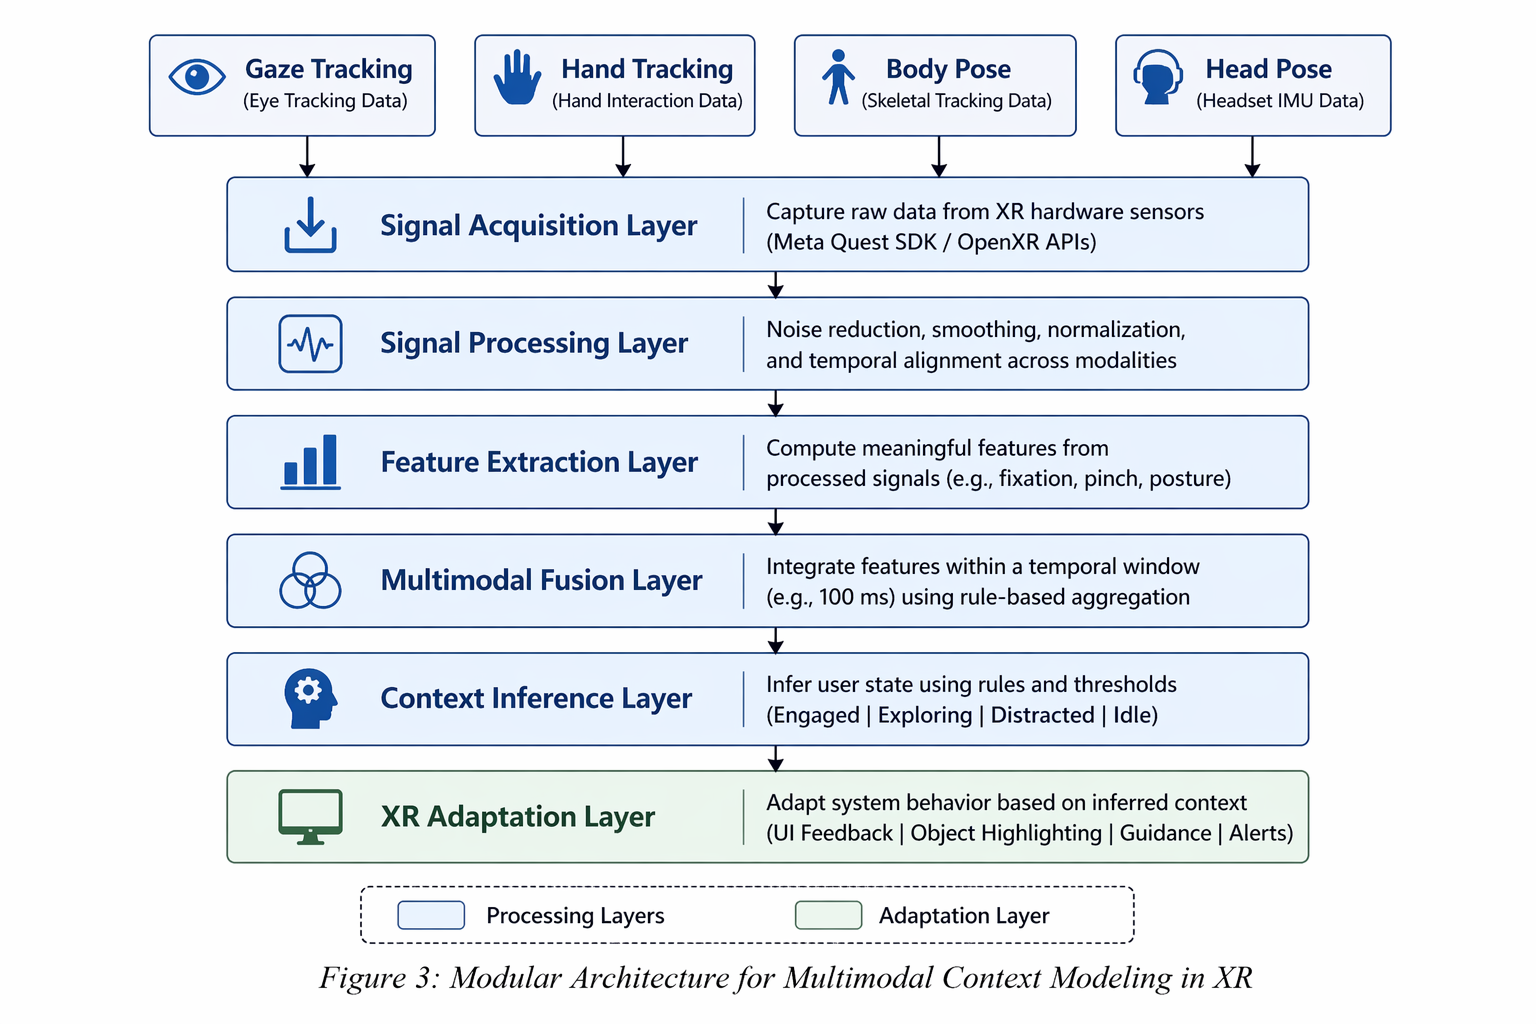
\includegraphics[width=0.9\textwidth]{figures/figure3_architecture.png}
  \caption{Reference modular architecture figure from the earlier draft. The conceptual layering remains useful and is consistent with the current implementation, although the final paper uses the repository terminology of Sensor Abstraction, Context Engine, and XR Adaptation / App Shell.}
  \label{fig:architecture}
\end{figure*}

\section{Methodology}
\subsection{Task Environment}
The application scene is a short sorting simulation implemented as \texttt{TrainingSimulation}. The user is presented with three task objects, a cube, cylinder, and sphere, which must be placed in the correct receptacles. Task objects and receptacles are tagged as Areas of Interest (AOIs), enabling the gaze subsystem to identify when task-relevant objects are being inspected. The scene is intentionally simple because the goal is not to study game mechanics but to isolate context inference during focused interaction.

\subsection{Signal Acquisition}
\subsubsection{Gaze and AOI Detection}
The current repository implementation resolves a gaze ray using the center-eye camera or center-eye anchor and casts the ray into the scene against AOI colliders. This produces gaze origin, normalized gaze direction, AOI hit name, a placeholder fixation estimate in Layer 1, and a rendered debug ray for QA. The code comments state that this update path runs in Unity \texttt{Update()} to follow headset refresh behavior at approximately 60--90 Hz.

\subsubsection{Head and Body Signals}
Head pose is captured from the main camera or OVR camera rig. Body pose capture uses \texttt{OVRSkeleton} joints and computes head position, head forward vector, head-gaze divergence, a coarse posture class, spine angle, and average joint velocity. The current Layer 1 posture labels are \texttt{standing}, \texttt{leaning}, \texttt{reaching}, and \texttt{unknown}, produced from spine-angle heuristics.

\subsubsection{Hand Interaction Signals}
Hand capture reads \texttt{OVRHand} input and controller fallback input. Pinch events are detected using a pinch-strength threshold of 0.7, and interaction counts are accumulated over a ten-second sliding window. The hand subsystem also computes the distance between the dominant tracked hand and the nearest AOI-tagged object.

\subsubsection{Spatial Context Signals}
Spatial context detection updates every five seconds and estimates \texttt{boundary\_type} (\texttt{stationary}, \texttt{room\_scale}, \texttt{custom}, or \texttt{passthrough}) and \texttt{posture\_mode} (\texttt{sitting}, \texttt{standing}, or \texttt{room\_scale}). Boundary type is inferred from the configured guardian geometry area. Posture mode is inferred from headset height relative to a session calibration point, with a sitting threshold difference of 0.25 m.

\subsection{Signal Synchronization}
The \texttt{SignalSynchroniser} collects the latest values from all capture scripts and writes them into a single \texttt{SignalFrame} every 100 ms. Missing values fall back to the most recent valid values or safe defaults. The current implementation does not yet expose an explicit per-signal staleness flag, which was requested in the implementation guide; this gap should be acknowledged as a limitation.

\subsection{Feature Extraction}
Feature extraction occurs in Layer 2 and converts raw frame values into inference-oriented features.

\paragraph{Gaze Features.}
\texttt{GazeFeatureExtractor} computes \texttt{currently\_on\_task\_aoi}, \texttt{fixation\_on\_aoi}, \texttt{fixation\_duration\_s}, \texttt{head\_gaze\_divergence\_deg}, \texttt{aoi\_dwell\_ratio}, and \texttt{saccade\_rate\_per\_s}. The current implementation uses an I-VT velocity threshold of 30 deg/s, a minimum fixation duration of 80 ms \cite{salvucci2000}, a 2000 ms saccade window, and a 5000 ms AOI dwell window.

\paragraph{Body Features.}
\texttt{BodyFeatureExtractor} maps raw posture and spine-angle values into \texttt{Upright}, \texttt{LeaningForward}, \texttt{Slouched}, and \texttt{LeaningBack}, and also passes forward average joint velocity.

\paragraph{Hand Features.}
\texttt{HandFeatureExtractor} computes interaction frequency as \texttt{interaction\_count\_10s / 10}, object proximity as \texttt{nearest\_object\_dist\_m < 0.3}, and pinch activity as the logical OR of left and right pinch states.

\paragraph{Spatial Features.}
\texttt{SpatialContextExtractor} computes posture mode, boundary type, and locomotion activity. Locomotion is discretized from inter-frame head movement using the thresholds \(< 0.1\) m (\texttt{None}), \(< 0.5\) m (\texttt{Low}), and \(\geq 0.5\) m (\texttt{Active}).

\subsection{Context State Definition}
User context is inferred as one of four discrete behavioral states derived from multimodal feature integration. Each state represents a distinct level of attention, engagement, and interaction activity. States are determined by rule-based logic that evaluates integrated features within a temporal window, ensuring real-time classification and interpretability for downstream adaptive behaviors.

\subsubsection{Engaged}
\textbf{Definition:} User is actively interacting with task-relevant objects while maintaining focused visual attention and stable posture.

\textbf{Measurable criteria:} In the stronger reference formulation from the earlier draft, the Engaged state is associated with fixation on task-relevant AOIs, AOI dwell ratio above 0.6, interaction frequency above 0.1, posture within \{Upright, LeaningForward\}, and low head-gaze divergence. The current repository implementation uses a slightly more implementation-specific rule that combines task-AOI focus, fixation or active interaction, supportive posture, room-scale engagement cues, head-gaze divergence \(\leq 18^\circ\), and saccade rate \(\leq 2.5/s\).

\subsubsection{Distracted}
\textbf{Definition:} User attention has deviated from task-relevant elements, interaction has reduced or ceased, and head orientation indicates attention drift.

\textbf{Measurable criteria:} In the stronger reference formulation, the Distracted state corresponds to no fixation on AOI, AOI dwell ratio below 0.3, head-gaze divergence above \(20^\circ\), and minimal hand interaction. The current repository implementation uses a more concrete implementation rule based on not being on task AOI, no fixation on task AOI, AOI dwell below 0.20, away-signals from divergence or saccade activity or body movement, no active pinch, and low interaction frequency.

\subsubsection{Transitioning}
\textbf{Definition:} User is shifting attention between tasks or preparing to engage with a new target.

\textbf{Measurable criteria:} The reference draft defined this state using either head-gaze divergence above \(15^\circ\) or combined posture change plus rising interaction. The current repository implementation captures a broader transitional pattern including high head-gaze divergence, task-adjacent but unstable gaze, short fixations, moderate AOI dwell, or preparatory hand proximity.

\subsubsection{Idle}
\textbf{Definition:} User has ceased all activity across all modalities and has maintained inactivity for a sustained duration.

\textbf{Measurable criteria:} The reference draft specifies average joint velocity below 0.05, zero interaction frequency, and no fixation on AOI for at least 5 seconds. The current repository implementation uses low body movement, no effective hand activity, no object proximity, no task-directed gaze, and very low AOI dwell.

\subsection{Rule-Based Fusion and Hysteresis}
The current \texttt{ContextFusionEngine} applies prioritized rules to infer a candidate state. Each inferred state receives a confidence score initialized from 0.5 and incremented based on supporting multimodal evidence, then clamped to the range \([0,1]\). The \texttt{ContextStateMachine} reduces oscillation through a minimum state hold time of 0.5 s and a pending confirmation time of 0.2 s.

\begin{figure}[t]
  \centering
  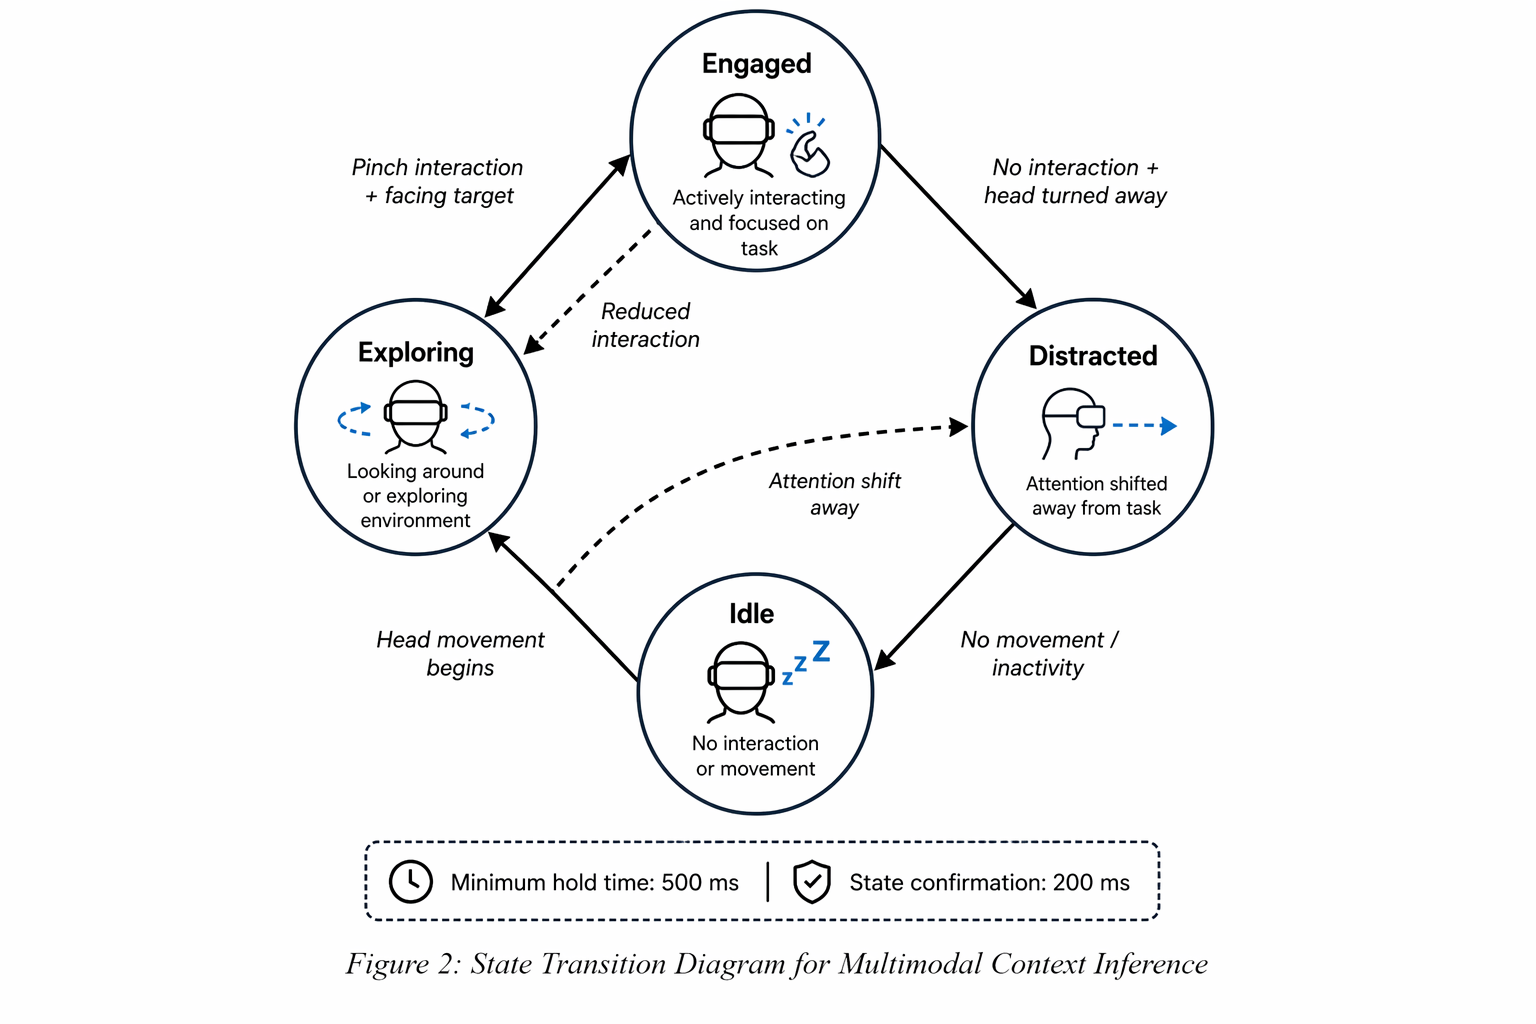
\includegraphics[width=\columnwidth]{figures/figure2_state_reference.png}
  \caption{Reference state-transition diagram from the earlier draft. The older figure uses the label \textit{Exploring}; in the current repository this behavior is represented by the implemented \textit{Transitioning} state and related task-shift logic.}
  \label{fig:state}
\end{figure}

\section{Implementation}
\subsection{Software Stack}
The repository currently documents the following versions:
\begin{itemize}[leftmargin=1.2em]
  \item Unity Editor: 2022.3.62f1
  \item OpenXR Plugin: 1.14.3
  \item Meta XR All-in-One SDK: 201.0.0
  \item Meta XR Core SDK: included with Meta XR All-in-One SDK
  \item OVRPlugin: 1.201.0
\end{itemize}

\subsection{Runtime Integration}
The \texttt{XRAppShellController} binds the context source to the application layer, publishes \texttt{XRContextSnapshot} updates, aligns the training simulation in front of the user, and provides fallback simulation behavior for QA. If the live context source cannot be found and fallback is enabled, the system can publish simulated states for manual testing.

\subsection{Task Logic}
The task layer uses \texttt{ReceptacleTrigger}, \texttt{SortableTaskObject}, and \texttt{TrainingSimulationTaskManager}. Correct placements are counted, and the task completes when all three objects are sorted.

\subsection{Adaptive Behaviors}
\texttt{AdaptationManager} maps current state and boundary type into adaptive behavior variants:
\begin{itemize}[leftmargin=1.2em]
  \item Engaged: subtle vignette and reduced unnecessary hints
  \item Distracted: visual nudge, spatial audio cue, or minimal overlay depending on boundary mode
  \item Transitioning: next-task preload or content repositioning
  \item Idle: rest panel, continue / break / recenter controls, and optional floor arrow
\end{itemize}

\subsection{Logging}
\texttt{ContextLogger} writes each processed frame to a timestamped \texttt{.jsonl} file under \texttt{Application.persistentDataPath}. Logged entries include full signal-frame payload, context state, confidence, previous state, hold duration, state-transition count, and nearest interactable reference.

\section{Evaluation Design}
This section reflects the required empirical paper design from the implementation guide and WBS. Replace placeholders with the real study details before submission.

\subsection{Study Design}
The planned study is a within-subjects comparison with two conditions:
\begin{itemize}[leftmargin=1.2em]
  \item \textbf{Baseline condition:} system active, adaptive behaviors disabled
  \item \textbf{Adaptive condition:} full multimodal inference and adaptive behaviors enabled
\end{itemize}
Condition order should be counterbalanced across participants.

\subsection{Participants}
Target participants: 8--10. Minimum usable sample for inferential analysis: 6.

\subsection{Procedure}
Each participant session is planned as follows:
\begin{enumerate}[leftmargin=1.2em]
  \item Consent and briefing
  \item Familiarization with headset and sorting task
  \item Condition A or B (8--12 minutes)
  \item NASA-TLX and self-report ratings
  \item Five-minute break
  \item Remaining condition
  \item NASA-TLX and self-report ratings
  \item Debrief
\end{enumerate}

\subsection{Measures and Analysis}
The primary measure is context detection accuracy against participant self-report or ground-truth labeling. Secondary measures are task completion time, number of sorting errors, NASA-TLX workload score, and subjective engagement and distraction ratings. The implementation guide specifies descriptive summaries, a confusion matrix for state classification, and a Wilcoxon signed-rank test for Adaptive vs Baseline comparisons.

\section{Current Project Status for the Paper}
Considering the old draft only as reference, the current project is no longer just a concept draft. The repository now contains a real implemented pipeline for the paper's core technical claim: signal schema, synchronization, feature extraction, rule-based fusion, state hysteresis, XR adaptation, task progression, and JSONL logging are all present in code. Therefore, the paper can now strongly support the architecture, methodology, and implementation sections.

What remains incomplete for a fully submission-ready empirical paper is the evidence layer: the final user-study results, the complete participant and ethics details, and the full verified related-work bibliography from the older draft. In other words, the system side is substantially stronger than before, while the evaluation side still needs completion.

\section{Discussion}
The intended interpretation of the system is that multimodal sensing provides a more meaningful representation of user context than isolated XR signals. The design of the prototype supports this claim at the system-architecture level because it combines attention, posture, interaction, and spatial setup before selecting adaptive support. The adaptive layer is deliberately lightweight: the goal is not to interrupt the user but to provide support that matches inferred state.

From an HCI perspective, the most important design principle in the current prototype is not the specific threshold values but the explicit separation between sensing, inference, and application behavior. This separation improves inspectability, modularity, and future extensibility. It also creates a path toward a plugin-style architecture in which the context engine can later be replaced by a learned model without rewriting the XR application layer.

\section{Limitations}
Several limitations should be stated explicitly in the final paper. First, the current repository implementation is still a proof-of-concept. Second, the current task is deliberately simple, so ecological validity for richer training workflows remains limited. Third, the fusion model is manually authored and threshold-driven, which improves interpretability but may reduce generalization. Fourth, the current repository does not yet include explicit per-signal staleness flags, even though the implementation guide proposed them. Fifth, the current gaze implementation in the repository is a center-eye gaze-ray approximation rather than a fully documented hardware eye-tracking pipeline; the paper should not overclaim beyond the implemented code path. Finally, the complete bibliography from the older draft and the final empirical results are not yet available in machine-readable form, so those elements still require restoration.

\section{Future Work}
The planning documents identify several extensions that should be preserved in the final manuscript: locomotion-aware context refinement, face-tracking integration, EEG or physiological augmentation, multi-user or shared-space support, and personalization of thresholds and adaptation policies. An important near-term next step is the creation of a labeled session dataset from the current logging pipeline. That dataset would support direct comparison between the current rule-based engine and future learned classifiers.

\section{Conclusion}
GazePose-Context presents a structured XR prototype for multimodal context inference and adaptive training support. The system combines gaze, head, body, hand, and spatial context signals inside a three-layer Unity architecture and maps the resulting inferred states to lightweight, boundary-aware adaptive behavior. The repository already supports synchronized signal capture, feature extraction, rule-based fusion, state stabilization, runtime adaptation, and persistent logging. This LaTeX paper version updates the manuscript into paper-ready format, integrates the current implementation status and available reference materials, and is ready for further refinement once the remaining verified references and final study results are supplied.

\section*{Acknowledgments}
This research used AI-assisted tools in the following capacities: Claude for paper drafting assistance and research synthesis; GitHub Copilot for Unity C\# code scaffolding, with all generated code tested and validated on hardware by the researchers; literature-discovery tools for reference discovery; transcription tools for interview transcription if applicable; and charting tools for results figure generation. All scientific claims, research contribution statements, experimental results, and final citations were produced and verified by the human authors.

\begin{thebibliography}{9}

\bibitem{moreno2024}
Moreno-Arjonilla et al.,
``Eye-tracking on Virtual Reality: A Survey,''
\textit{Virtual Reality}, 2024.

\bibitem{long2024}
Long et al.,
``Multimodal Detection of External and Internal Attention in Virtual Reality using EEG and Eye Tracking,''
\textit{MuC}, 2024.

\bibitem{gazecomparison2020}
``Comparison of Gaze Accuracy and Precision in Real-World and Virtual Reality,''
\textit{Virtual Reality Journal}, 2020.

\bibitem{rakkolainen2021}
J. Rakkolainen et al.,
``Technologies for Multimodal Interaction in Extended Reality---A Scoping Review,''
\textit{Multimodal Technologies and Interaction}, 2021.

\bibitem{bustamante2025}
Bustamante et al.,
``Skeleton-Based Posture Recognition for Home Care,''
\textit{Expert Systems}, 2025.

\bibitem{neidhardt2023}
Neidhardt et al.,
``VR-based Body Tracking to Stimulate Musculoskeletal Training,''
\textit{arXiv}, 2023.

\bibitem{davari2024}
Davari and Bowman,
``Towards Context-Aware Adaptation in Extended Reality,''
\textit{arXiv}, 2024.

\bibitem{kim2026}
Kim et al.,
``From Controllers to Multimodal Input: XR Interaction Evolution,''
\textit{Sensors}, 2026.

\bibitem{ramiotis2025}
Ramiotis and Mania,
``CONTEXT-GAD: Context-Aware Gaze Adaptive Dwell Model,''
\textit{VRST}, 2025.

\bibitem{lei2023}
Lei et al.,
``A Novel Sensor Fusion Approach for Precise Hand Tracking in VR,''
\textit{Biomimetics}, 2023.

\bibitem{salvucci2000}
D. D. Salvucci and J. H. Goldberg,
``Identifying fixations and saccades in eye-tracking protocols,''
\textit{Proceedings of the 2000 Symposium on Eye Tracking Research \& Applications},
pp. 71--78, 2000.
doi: \url{https://doi.org/10.1145/355017.355028}

\bibitem{hart1988}
S. G. Hart and L. E. Staveland,
``Development of NASA-TLX (Task Load Index): Results of empirical and theoretical research,''
in \textit{Advances in Psychology}, vol. 52,
P. A. Hancock and N. Meshkati, Eds.
Amsterdam, The Netherlands: North-Holland, 1988, pp. 139--183.

\end{thebibliography}

\end{document}
